\begin{figure}[H]
\centering
\usetikzlibrary{positioning, fit, calc}   
  
\tikzset{block/.style={draw, thick, text width=2.5cm ,minimum height=1.1cm, align=center},   
line/.style={-latex}     
}  
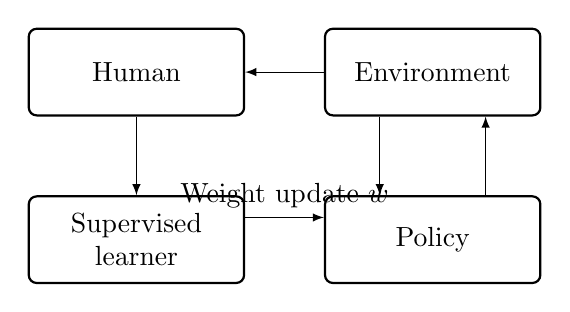
\begin{tikzpicture}  
\node[block, rounded corners=0.1cm] (human) {Human};  
\node[block,right=of human, rounded corners=0.1cm] (env) {Environment};   
\node[block, below=of env, rounded corners=0.1cm] (policy) {Policy}; 

\node[block, below=of human, rounded corners=0.1cm] (sup) {Supervised learner};  

 \draw[line] (env)-- (human);  
 %\draw[line] (policy)-- (env);  
% \draw[line] (env)-- (policy);  
 %\draw[->] (policy.140) -- (env.220);
 %\draw[->] (env.60) -- (policy.300);
 
 %\draw[red, very thick] (env.80)-- ++(1.3cm,1.3cm);
 \draw[line](env.220) -- (policy.140);
\draw[line](policy.40) -- (env.320);
\draw[line] ($(sup.north east)!0.25!(sup.south east)$) -- node[above] {Weight update $w$} ($(policy.north west)!0.25!(policy.south west)$);
 \draw[line](human.south) -- (sup.north);
    
\end{tikzpicture}  
\caption{Autoencoder, \cite{Autoencoder-tikz}} \label{fig:autoencoder}
\end{figure}
